% Asset ID: A21BinomialExpansionTikZ-005
% Unit: A21
% Topic code: A21-SS
% Topic ID: A21BinomialExpansion
% Purpose: Partial fractions workflow
\documentclass[tikz,border=10pt]{standalone}
\usepackage{amsmath}
\usetikzlibrary{arrows.meta,positioning}
\begin{document}
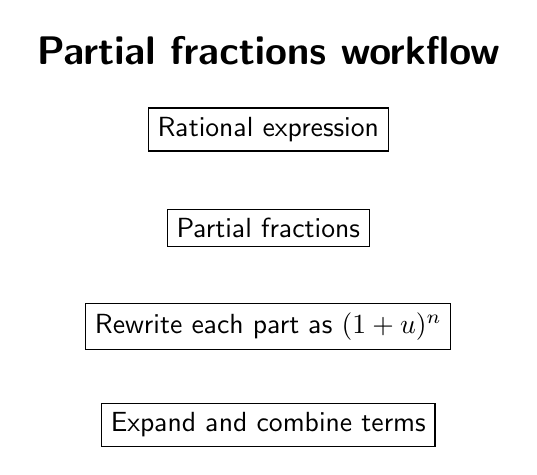
\begin{tikzpicture}[every node/.style={font=\sffamily}]
\node[font=\sffamily\bfseries\Large] at (0,3) {Partial fractions workflow};
\node[draw,align=center] at (0,2) {Rational expression};\node[draw,align=center] at (0,0.75) {Partial fractions};\node[draw,align=center] at (0,-0.5) {Rewrite each part as $(1+u)^n$};\node[draw,align=center] at (0,-1.75) {Expand and combine terms};
\end{tikzpicture}
\end{document}
